\documentclass[runningheads]{llncs}

\usepackage[T1]{fontenc}
\usepackage{amsmath,amssymb}
\usepackage{booktabs}
\usepackage{array}
\usepackage{graphicx}
\usepackage{xcolor}
\usepackage{lmodern}
\usepackage{tikz}
\usetikzlibrary{arrows.meta,positioning,shapes.geometric,fit,backgrounds}
\usepackage{hyperref}
\hypersetup{hidelinks,colorlinks=true,allcolors=blue!60!black}

\renewcommand{\topfraction}{0.95}
\renewcommand{\bottomfraction}{0.85}
\renewcommand{\textfraction}{0.1}
\renewcommand{\floatpagefraction}{0.80}
\setlength{\textfloatsep}{6pt plus 1pt minus 1pt}
\setlength{\floatsep}{6pt plus 1pt minus 1pt}
\setlength{\intextsep}{6pt plus 1pt minus 1pt}

\newcommand{\method}{ESV-Gap}
\newcommand{\runid}{\texttt{deep\_learning\_\allowbreak iot\_intrusion\_\allowbreak de\_20260831\_\allowbreak 114802}}
\newcolumntype{L}[1]{>{\raggedright\arraybackslash}p{#1}}
\providecommand{\doi}[1]{}
\renewcommand{\doi}[1]{\href{https://doi.org/#1}{\texttt{\scriptsize doi:#1}}}

\begin{document}

\title{ESV-Gap: An Auditable Autonomous Reasoning Architecture for Evidence-Grounded Scientific Hypothesis Triage}
\titlerunning{Auditable Hypothesis Triage with ESV-Gap}

\author{Anonymous Author(s)}
\authorrunning{Anonymous Author(s)}
\institute{Anonymous Institution / Laboratory\\
\email{anonymous@conference-review.net}}

\maketitle

\begin{abstract}
Autonomous machine intelligence (AMI) agents increasingly formulate scientific hypotheses by detecting associative patterns in literature, but can conflate representation sparsity with scientific novelty. We present \method{}, an auditable autonomous reasoning architecture executing a fail-closed epistemic control loop: \textbf{Observe} $\rightarrow$ \textbf{Hypothesize} $\rightarrow$ \textbf{Verify} $\rightarrow$ \textbf{Reason} $\rightarrow$ \textbf{Decide} $\rightarrow$ \textbf{Act/Abstain}. \method{} replaces naive graph sparsity heuristics with a Four-Pillar Evidence Verification engine: (A) two-stage external counterevidence verification decoupling lexical retrieval from semantic relation extraction; (B) source-disjoint author corroboration; (C) empirical extractor diagnostics reporting precision, recall, and miss rate with Wilson 95\% confidence intervals; and (D) corpus coverage diagnostics via Heaps' law and marginal discovery decay. In an empirical case study on deep-learning IoT intrusion detection (150 retained publications, 1,404 relation events, 1,185 canonical entities), \method{} triaged five post-gate candidate hypotheses: three were semantically refuted by verified recent counterevidence ($60\%$), one was escalated to human review due to circular provenance, and one was qualified as an evidence-supported open hypothesis corroborated by three independent 2026 publications, preventing $80\%$ ($4/5$) from premature promotion. Diagnostic extractor evaluation revealed an empirical miss rate of $22.2\%$ ($95\%$ Wilson CI: $[11.7\%, 38.1\%]$), while canonical vocabulary growth ($\beta = 0.995$, discovery decay $-10.3\%$) established an unsaturated corpus. Across six deterministic fault-injection scenarios, \method{} enforced $100\%$ fail-closed abstention.

\keywords{Autonomous Machine Intelligence \and Evidence-Grounded Reasoning \and Scientific Discovery Agents \and Knowledge Graphs \and Hypothesis Triage \and Fail-Closed Systems.}
\end{abstract}

\section{Introduction}
\label{sec:intro}

Autonomous Machine Intelligence (AMI) aims to realize artificial agents capable of acquiring knowledge, reasoning over open-world dynamics, formulating hypotheses, and executing goal-directed plans with bounded human intervention~\cite{langley1987,king2009automation,lecun2022path}. While foundation models and agentic workflows enable automated discovery systems to scan literature and propose hypotheses at scale~\cite{aiscientist2024}, generative capacity has outpaced epistemic self-verification. Generating plausible conjectures is computationally cheap; determining whether a proposition represents a genuine open question, an already solved problem, an artifact of incomplete retrieval, or an extractor error is the central epistemic bottleneck~\cite{wadden2020scifact,schneider2022decade}.

When an autonomous agent constructs a scientific knowledge graph (KG), an absent edge between a method and an application can trigger a candidate research-gap hypothesis. Yet edge absence stems from multiple failure modes: unindexed external literature, relation extraction errors, terminology fragmentation, or abstract-level truncation. As Altman and Bland formulated, \emph{``Absence of evidence is not evidence of absence''}~\cite{altman1995absence}. Equating representation sparsity with scientific novelty can yield false-positive gap claims, duplicate research, and misallocated experimental effort.

This paper addresses a critical challenge in Autonomous Machine Intelligence: \textbf{How can an autonomous agent rigorously determine whether an internally generated scientific hypothesis is sufficiently supported by external evidence to justify downstream formulation, or whether it must autonomously abstain?}

We present \textbf{\method{}}, an auditable autonomous reasoning architecture for evidence-grounded hypothesis triage. Rather than treating hypothesis generation as an unconstrained generative task or defaulting to link prediction on a static graph, \method{} frames hypothesis triage as an active epistemic control loop:
\begin{equation}
\label{eq:loop}
\text{Observe} \longrightarrow \text{Hypothesize} \longrightarrow \text{Verify} \longrightarrow \text{Reason} \longrightarrow \text{Decide} \longrightarrow \text{Act/Abstain}
\end{equation}

\noindent\textbf{Key Contributions.} This work makes five primary contributions:
\begin{enumerate}\setlength{\itemsep}{0pt}\setlength{\topsep}{2pt}\setlength{\parsep}{0pt}\setlength{\partopsep}{0pt}
  \item \textbf{Two-Stage External Verification (Pillar A):} We decompose Pillar A into lexical candidate retrieval (Stage A1) and semantic relation extraction (Stage A2), preventing mere co-mentions of limitations from falsely refuting candidate gaps.
  \item \textbf{Strict Source-Disjoint Corroboration (Pillar B):} We formalize graph provenance verification requiring independent, author-disjoint literature in the local corpus ($\mathcal{P}_{\text{cand}} \cap \mathcal{P}_{\text{corrob}} = \emptyset$), excluding circular citations from corroboration and routing candidates without independent support to review.
  \item \textbf{Diagnostic Reliability Characterization (Pillars C \& D):} We replace unjustified global bounds with empirical extractor diagnostics ($n=36$, Wilson 95\% CIs) and track canonical vocabulary growth via Heaps' law and marginal discovery decay.
  \item \textbf{Decoupled Epistemic Control Policy:} We separate disposition space $\mathcal{D}$ from action space $\mathcal{A}$ via a deterministic policy $\pi: \mathcal{D} \rightarrow \mathcal{A}$, providing an auditable, fail-closed abstention mechanism.
  \item \textbf{Empirical Auditability and Fault-Injection Validation:} We evaluate \method{} on 150 IoT cybersecurity publications, retaining complete record-level verification traces for all inspected external documents in the reproducibility artifact (\runid{}) and demonstrating 100\% fail-closed abstention across six predefined failure modes.
\end{enumerate}

\section{Related Work}
\label{sec:related}

\noindent\textbf{Autonomous Scientific Discovery and AMI.} Early symbolic systems such as BACON~\cite{langley1987} and the Robot Scientist Adam~\cite{king2009automation} executed closed-loop hypothesis generation and physical experimentation. In modern AMI, LeCun~\cite{lecun2022path} formalizes autonomous agents around perception, world modeling, reasoning, and objective-driven control. Recently, LLM-based systems such as The AI Scientist~\cite{aiscientist2024} demonstrated automated literature review and ideation. However, existing generative agents lack verifiable epistemic self-assessment and can accept unsupported or previously resolved gaps when external verification is absent.

\noindent\textbf{Graph-Theoretic Gap Discovery.} Knowledge graphs provide structured representations for literature synthesis and hypothesis discovery~\cite{swanson1986fish,schneider2022decade,chen2019ukge}. Most closely related to our work, Dachepally and Kandasamy~\cite{rahul2026dynamic} generated gap candidates using TransE link prediction, Louvain community detection~\cite{blondel2008fast}, and temporal activity decay. While their work offers valuable techniques for initial graph candidate generation, \method{} addresses the downstream verification problem: determining whether a structurally plausible candidate remains defensible after external retrieval, semantic counterevidence analysis, provenance checks, and corpus-coverage diagnostics.

\noindent\textbf{Scientific Claim Verification.} Claim verification frameworks, such as SciFact~\cite{wadden2020scifact} and SciFact-Open~\cite{wadden2022scifactopen}, evaluate natural-language assertions against corpora. However, these systems verify factual assertions (e.g., entity properties) rather than epistemic research gaps asserting that a capability has not been achieved. Verifying negative gap claims requires open-world external retrieval and semantic verification of whether retrieved papers resolve or merely discuss the challenge.

\noindent\textbf{Selective Classification and Fail-Closed Systems.} In high-stakes decision systems, rejecting predictions under insufficient evidence is essential~\cite{saltzer1975protection,shneiderman2020hcai}. Selective classification and learning with rejection~\cite{cortes2016learning,geifman2017selective} formalize coverage-error trade-offs through an explicit abstention action. \method{} operationalizes this fail-safe principle: when external index probes fail, data is malformed, or corroboration is circular, the agent autonomously abstains and escalates to human review.

\section{Problem Formulation and Control Loop}
\label{sec:problem}

\subsection{Knowledge Graph and Attributed Relation Events}
Let $\mathcal{P} = \{p_1, \dots, p_N\}$ be a bounded corpus of ingested publications. We construct a multigraph $\mathcal{G} = (\mathcal{E}, \mathcal{R}, \mathcal{E}_{\text{events}})$ where $\mathcal{E}$ denotes canonical entities and $\mathcal{R}$ denotes directed relations (\texttt{ADDRESSES}, \texttt{USES}, \texttt{EVALUATES\_ON}, \texttt{IMPROVES}, \texttt{LACKS}, \texttt{APPLIED\_\allowbreak TO}). Each extracted instance is a \textbf{directed attributed relation event} $e = \langle u, r, v, p, y, c, q \rangle$, where $u, v \in \mathcal{E}$, $r \in \mathcal{R}$, $p \in \mathcal{P}$ is the source paper, $y \in \mathbb{N}$ is publication year, $c \in [0, 1]$ is confidence, and $q$ is the verbatim evidence span.

\subsection{Operational Hypothesis vs. Global Scientific Absence}
In naive graph discovery, an unobserved link between method $u$ and capability $v$ is asserted as an absolute gap: $\Phi_{\text{absent}}(u, v) \equiv \neg \exists e \in \mathcal{E}_{\text{events}} : \text{subj}(e) = u \wedge \text{rel}(e) = \texttt{ADDRESSES} \wedge \text{obj}(e) = v$. Such global absence claims cannot be established from a bounded corpus alone. We reformulate gap triage as an \textbf{operational verification claim}:
\begin{definition}[Operational Hypothesis Claim]
Given candidate gap $h = \langle u, \texttt{LACKS}, v \rangle$, external index family $\mathcal{S}$, query family $\mathcal{Q}(h)$, semantic verifier $\mathcal{V}$, and timestamp $t$, the machine-testable proposition is:
\begin{equation}
\label{eq:operational_claim}
\Phi_{\text{op}}(h) \equiv \text{Complete}(h) \wedge \left( \mathcal{C}_{\text{verified}}(h) = \emptyset \right) \wedge \left( |\mathcal{P}_{\text{disjoint}}(h)| \ge 1 \right)
\end{equation}
where $\mathcal{C}_{\text{verified}}$ is verified external counterevidence, $\mathcal{P}_{\text{disjoint}}$ is source-disjoint corroboration, and $\text{Complete}(h) \in \{0, 1\}$ indicates verification completion. Here, $\text{Complete}(h) = 1$ iff all configured index queries $\mathcal{S}$ and semantic checks $\mathcal{V}$ execute successfully without timeouts, HTTP 429 throttling, malformed JSON, or missing evidence spans. If any mandatory verification step fails, $\text{Complete}(h) = 0$, ensuring external failure cannot be conflated with evidence of absence.
\end{definition}

\subsection{Evidence, Dispositions, and Control Action Space}
Let $\mathbf{e}(h) = \langle \text{Complete}(h), |\mathcal{C}_{\text{verified}}(h)|, |\mathcal{P}_{\text{disjoint}}(h)|, \text{CorpusVerdict}(\mathcal{P}), R_{\text{ext}} \rangle$ denote the Four-Pillar evidence vector. Hypothesis triage is formalized via decision rule $\delta: \mathbf{e}(h) \rightarrow \mathcal{D}$ and action policy $a(h) = \pi(\delta(h))$ under fail-closed precedence:
\begin{equation}
\label{eq:disposition}
\delta(h) = \begin{cases}
\text{\scriptsize REFUTED}, & \text{if } |\mathcal{C}_{\text{verified}}(h)| \ge 1 \\
\text{\scriptsize REVIEW\_REQUIRED}, & \text{if } \text{Complete}(h) = 0 \;\vee\; |\mathcal{P}_{\text{disjoint}}(h)| < 1 \\
\text{\scriptsize EVIDENCE\_SUPPORTED}, & \text{if } \Phi_{\text{op}}(h) \wedge \text{CorpusVerdict}(\mathcal{P}) = \text{\scriptsize SATURATED} \\
\text{\scriptsize SUPPORTED\_OPEN}, & \text{if } \Phi_{\text{op}}(h) \wedge \text{CorpusVerdict}(\mathcal{P}) \ne \text{\scriptsize SATURATED}
\end{cases}
\end{equation}
The policy $\pi: \mathcal{D} \rightarrow \mathcal{A}$ executes: $\text{\scriptsize REFUTED} \mapsto \text{\scriptsize REJECT}$, $\text{\scriptsize REVIEW\_REQUIRED} \mapsto \text{\scriptsize ABSTAIN\_AND\_ESCALATE}$, $\text{\scriptsize EVIDENCE\_SUPPORTED} \mapsto \text{\scriptsize RETAIN\_AND\_FORMULATE}$, and $\text{\scriptsize SUPPORTED\_OPEN} \mapsto \text{\scriptsize RETAIN\_WITH\_WARNING}$. This establishes the closed loop $\mathbf{e}(h) \mapsto \delta(h) \mapsto a(h) = \pi(\delta(h))$. Because \texttt{REFUTED} has highest precedence, a single verified counterevidence record suffices for rejection regardless of completion status. If mandatory external verification remains incomplete and no verified counterevidence has already refuted the hypothesis, the decision rule returns \texttt{REVIEW\_REQUIRED} and triggers fail-closed abstention.

\section{\method{} Architecture}
\label{sec:arch}

The \method{} architecture operationalizes the epistemic loop of Eq.~(\ref{eq:loop}). As illustrated in Fig.~\ref{fig:arch}, the pipeline processes raw literature through structured observation, candidate generation, multi-stage verification, and policy execution.

\begin{figure}[t]
\centering
\resizebox{\columnwidth}{!}{%
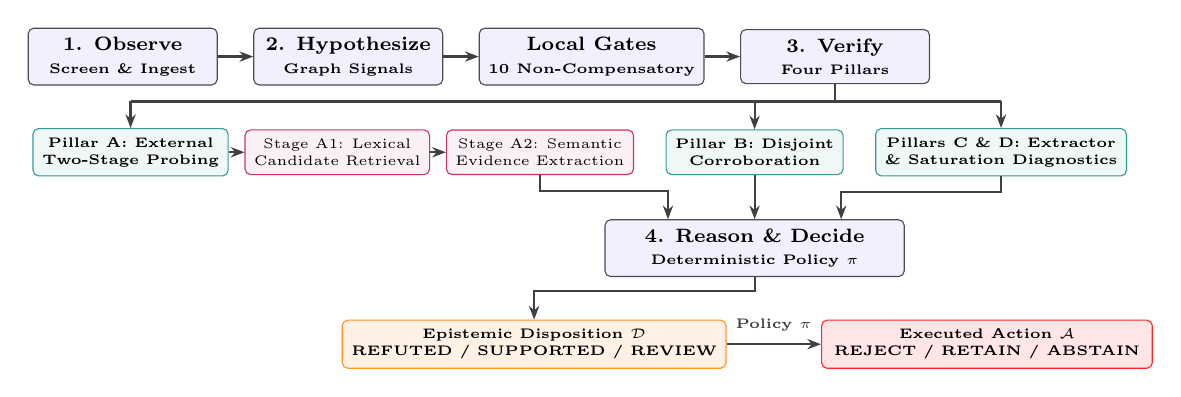
\begin{tikzpicture}[
  box/.style={rectangle, draw=black!70, fill=blue!6, rounded corners=2pt, minimum width=2.4cm, minimum height=0.54cm, font=\scriptsize\bfseries, align=center},
  stagebox/.style={rectangle, draw=purple!80, fill=purple!6, rounded corners=2pt, minimum width=1.95cm, minimum height=0.50cm, font=\tiny, align=center},
  pillar/.style={rectangle, draw=teal!80, fill=teal!6, rounded corners=2pt, minimum width=2.1cm, minimum height=0.52cm, font=\tiny\bfseries, align=center},
  disp/.style={rectangle, draw=orange!85, fill=orange!10, rounded corners=2pt, minimum width=4.2cm, minimum height=0.58cm, font=\tiny\bfseries, align=center},
  act/.style={rectangle, draw=red!85, fill=red!10, rounded corners=2pt, minimum width=4.2cm, minimum height=0.58cm, font=\tiny\bfseries, align=center},
  arrow/.style={-{Stealth[scale=0.75]}, thick, color=black!75},
  bus/.style={thick, color=black!75}
]

% Tier 1: Operational Loop
\node[box] (obs) {1. Observe\\ \tiny Screen \& Ingest};
\node[box, right=0.45cm of obs] (hyp) {2. Hypothesize\\ \tiny Graph Signals};
\node[box, right=0.45cm of hyp] (gates) {Local Gates\\ \tiny 10 Non-Compensatory};
\node[box, right=0.45cm of gates] (ver) {3. Verify\\ \tiny Four Pillars};

\draw[arrow] (obs) -- (hyp);
\draw[arrow] (hyp) -- (gates);
\draw[arrow] (gates) -- (ver);

% Tier 2: Verification Pillars
\node[pillar, below=0.54cm of obs, xshift=0.1cm] (pila) {Pillar A: External\\ Two-Stage Probing};
\node[stagebox, right=0.2cm of pila] (stg1) {Stage A1: Lexical\\ Candidate Retrieval};
\node[stagebox, right=0.2cm of stg1] (stg2) {Stage A2: Semantic\\ Evidence Extraction};
\draw[arrow] (pila) -- (stg1);
\draw[arrow] (stg1) -- (stg2);

\node[pillar, right=0.4cm of stg2] (pilb) {Pillar B: Disjoint\\ Corroboration};
\node[pillar, right=0.4cm of pilb] (pilcd) {Pillars C \& D: Extractor\\ \& Saturation Diagnostics};

% Clean Distribution Bus from 3. Verify to Pillars
\coordinate (splitY) at ([yshift=-0.22cm]ver.south);
\draw[bus] (ver.south) -- (splitY);
\draw[bus] (pila.north |- splitY) -- (pilcd.north |- splitY);
\draw[arrow] (pila.north |- splitY) -- (pila.north);
\draw[arrow] (pilb.north |- splitY) -- (pilb.north);
\draw[arrow] (pilcd.north |- splitY) -- (pilcd.north);

% Tier 3: Reasoning Box (centered under Pillar B)
\node[box, below=0.56cm of pilb, minimum width=3.8cm] (rsn) {4. Reason \& Decide\\ \tiny Deterministic Policy $\pi$};

% Clean Inputs into 4. Reason & Decide without line intersections
\draw[arrow] (stg2.south) -- ++(0,-0.20) -| ([xshift=-1.1cm]rsn.north);
\draw[arrow] (pilb.south) -- (rsn.north);
\draw[arrow] (pilcd.south) -- ++(0,-0.20) -| ([xshift=1.1cm]rsn.north);

% Tier 4: Disposition and Action (centered under rsn)
\node[disp, below=0.54cm of rsn, xshift=-2.8cm] (dspace) {Epistemic Disposition $\mathcal{D}$\\ \tiny REFUTED / SUPPORTED / REVIEW};
\node[act, right=1.2cm of dspace] (aspace) {Executed Action $\mathcal{A}$\\ \tiny REJECT / RETAIN / ABSTAIN};

\draw[arrow] (rsn.south) -- ++(0,-0.18) -| (dspace.north);
\draw[arrow] (dspace.east) -- node[above=1pt, font=\tiny\bfseries] {Policy $\pi$} (aspace.west);

\end{tikzpicture}%
}
\caption{\method{} Epistemic Control Loop, detailing the Two-Stage Pillar A verification engine and decoupling Epistemic Dispositions $\mathcal{D}$ from Executed Control Actions $\mathcal{A}$.}
\label{fig:arch}
\end{figure}

\subsection{Local Pre-Screening: Ten Non-Compensatory Validation Gates}
Candidate gap signals generated from the multigraph (via link-absence heuristics and community boundaries) must satisfy ten non-compensatory local gates (Table~\ref{tab:gates}). Specifically, Gate~5 (Local Semantic Closure) inspects sliding sentence windows for action patterns (\texttt{CLOSURE\_ACTION\_PATTERN}, e.g., \emph{address}, \emph{mitigate}, \emph{solve}, \emph{secure}) while filtering out discussed limitations via negation cues (\texttt{NEGATED\_}\allowbreak\texttt{RESOLUTION\_}\allowbreak\texttt{PATTERN}, e.g., \emph{struggle to address}, \emph{limitation to overcome}). Unnegated action matches escalate candidates to \texttt{REVIEW\_\allowbreak REQUIRED} rather than silently pruning them, ensuring suspected local closure receives expert inspection. Following gating, candidates are ranked using normalized publication recency as a secondary heuristic rather than an eligibility filter.

\begin{table}[htbp]
\centering
\caption{The Ten Non-Compensatory Local Validation Gates in \method{}.}
\label{tab:gates}
\scriptsize
\setlength{\tabcolsep}{2.5pt}
\renewcommand{\arraystretch}{0.78}
\begin{tabular}{lp{3.4cm}p{1.8cm}p{2.2cm}p{1.7cm}}
\toprule
\textbf{Gate} & \textbf{Validation Purpose} & \textbf{Input Data} & \textbf{Pass Condition} & \textbf{Failure Action} \\
\midrule
1. Provenance & Verifies anchor entity origin & Text spans & Anchor count $\ge 1$ & Reject (orphan) \\
2. Specificity & Eliminates generic non-informative nodes & Canonical tokens & Length $\ge 2$, non-stop & Reject (generic) \\
3. Direct Edge & Prevents claiming solved links as gaps & Adjacency & Direct count $= 0$ & Reject (closed) \\
4. Subsumptive & Checks semantic \& taxonomy aliases & Alias mapping & No subsumed link & Reject (redundant) \\
5. Local Semantic & Probes local corpus with action patterns & Corpus text & No unnegated action & Escalate (review) \\
6. Path Diversity & Requires multi-hop evidence support & Multigraph paths & Disjoint paths $\ge 2$ & Reject (unstable) \\
7. Edge Stability & Assesses deletion perturbation resilience & Edge dropout & Survival $\ge 0.70$ & Reject (fragile) \\
8. Paper Dropout & Tests cluster document dependence & Paper bootstrap & Survival $\ge 0.65$ & Reject (single-doc) \\
9. Plausible Edge & Tests survival under link additions & Plausible pool & Survival $\ge 0.60$ & Reject (plausible) \\
10. Domain Align & Enforces cybersecurity problem scope & Domain taxonomy & Similarity $\ge 0.75$ & Reject (out-of-scope) \\
\bottomrule
\end{tabular}
\end{table}

\subsection{Pillar A: Two-Stage External Counterevidence Verification}
\label{sec:pillar_a}

A key failure mode in automated gap discovery is the false assumption that \textbf{lexical co-mention implies counterevidence}. For example, a query matching ``deep learning IDS'' and ``zero-day attacks'' may retrieve an abstract stating that zero-day attacks remain an unresolved challenge for deep-learning intrusion detection architectures. Such a statement supports the limitation rather than refuting it. Treating such a retrieval as refuting the candidate is a critical scientific error.

To resolve this, we decompose Pillar A into two distinct stages:

\noindent\textbf{Stage A1: Lexical Candidate Retrieval.} The agent constructs boolean probe queries $Q_{\text{probe}}(u, v) = \texttt{"}u\texttt{" AND "}v\texttt{"}$ targeting external indexing services $\mathcal{S}$ (Semantic Scholar~\cite{semanticscholar2023} and OpenAlex~\cite{openalex2022}). The provider returns raw hit totals ($N_{\text{raw}}$). The agent paginates and fetches up to $K_{\text{fetch}} = 5$ recent records, extracting the title, abstract, authors, year, and persistent identifier (DOI, OpenAlex ID, Semantic Scholar ID). These records constitute the \textbf{Potential Counterevidence Pool}. Co-mention filtering at Stage A1 \emph{never} directly assigns a \texttt{REFUTED} disposition.

\noindent\textbf{Stage A2: Semantic Counterevidence Verification.} For each record in the Potential Counterevidence Pool, the agent extracts candidate evidence spans and assesses the semantic relation between method $u$ and capability $v$ using Llama-3.3-70b-versatile via Groq configured for low-variance decoding ($\text{temperature} = 0.0$, seed 42). The model outputs a structured JSON schema: \texttt{classification}, \texttt{evidence\_}\allowbreak\texttt{span}, \texttt{confidence} $\in [0, 1]$, and \texttt{relation\_}\allowbreak\texttt{rationale}. Model-reported confidence is retained as audit metadata and does not directly enter the disposition policy; Stage A2 decisions are based on the categorical relation label together with verbatim evidence-span validation. We classify records into four mutually exclusive labels: (1)~\texttt{VERIFIED\_}\allowbreak\texttt{COUNTEREVIDENCE}, where the paper demonstrates, implements, or evaluates capability $v$ for method $u$ (relations \texttt{ADDRESSES}, \texttt{IMPROVES}, \texttt{EVALUATES\_}\allowbreak\texttt{ON}); (2)~\texttt{SUPPORTING\_}\allowbreak\texttt{LIMITATION}, where the paper identifies $v$ as an unresolved limitation (relation \texttt{LACKS}); (3)~\texttt{AMBIGUOUS}, discussing $u$ and $v$ without definitive resolution; or (4)~\texttt{IRRELEVANT}, reflecting superficial lexical co-occurrence. To prevent generative hallucinations, an automated verbatim substring check is enforced: an extracted \texttt{evidence\_}\allowbreak\texttt{span} is mandatory for positive relation claims (\texttt{VERIFIED\_}\allowbreak\texttt{COUNTEREVIDENCE} and \texttt{SUPPORTING\_}\allowbreak\texttt{LIMITATION}) and must be an exact substring of the title or abstract; otherwise, the span is discarded as ungrounded. For \texttt{AMBIGUOUS} and \texttt{IRRELEVANT} records, the absence of a relation-supporting span reflects semantic lack of evidence rather than system failure and does not invalidate verification. If JSON decoding fails, exponential backoff is applied (up to 3 retries). Failure modes are handled distinctly: (a)~a valid response with unclear semantic relation yields \texttt{AMBIGUOUS}; (b)~persistent schema failure (missing required JSON fields after retries) or network failure sets $\text{Complete}(h) = 0$, routing the candidate to \texttt{REVIEW\_REQUIRED} unless already \texttt{REFUTED} by verified counterevidence. Infrastructure failure is thus decoupled from semantic ambiguity. Only records confirmed as \texttt{VERIFIED\_}\allowbreak\texttt{COUNTEREVIDENCE} with verified verbatim spans can contribute to a \texttt{REFUTED} disposition. For auditability, every verification record persists the exact quoted span, relation label, model confidence, DOI, and retrieval timestamp.

\subsection{Pillar B: Source-Disjoint Author Corroboration}
To ensure that a surviving candidate is not an idiosyncratic claim from a single research group or an artifact of self-citation, Pillar B searches the retained local corpus ($\mathcal{P}$) for independent supporting publications asserting explicit research gaps (via extracted \texttt{LACKS} relation triples or curated gap phrase patterns). Let $\mathcal{P}_{\text{cand}}$ be the set of papers that originated the candidate gap. The candidate must be corroborated by a disjoint publication set: $\mathcal{P}_{\text{corrob}} \subseteq \mathcal{P}$ with $\mathcal{P}_{\text{corrob}} \cap \mathcal{P}_{\text{cand}} = \emptyset$ and $\text{Authors}(\mathcal{P}_{\text{corrob}}) \cap \text{Authors}(\mathcal{P}_{\text{cand}}) = \emptyset$. If all local supporting citations trace back to the candidate's origin publication, the corroboration is flagged as circular, failing the independence gate and forcing an immediate \texttt{REVIEW\_REQUIRED} disposition. External Stage A2 records are tracked independently and do not increment local corpus $N_{\text{corrob}}$.

\subsection{Pillar C: Extractor Diagnostic Reliability Characterization}
\label{sec:pillar_c}

An absent graph edge may simply reflect an extraction failure by the NLP pipeline. To quantify this risk, Pillar C conducts an empirical diagnostic evaluation against an expert-annotated gold standard $\mathcal{D}_{\text{gold}}$ consisting of 36 ground-truth relation events across 10 representative abstracts.

Let $TP$, $FP$, and $FN$ denote true positive, false positive, and false negative counts on the diagnostic benchmark. The empirical metrics are $\text{Precision} = \frac{TP}{TP + FP}$, $\text{Recall} = \frac{TP}{TP + FN}$, and $F_1 = \frac{2 \cdot \text{Precision} \cdot \text{Recall}}{\text{Precision} + \text{Recall}}$. The empirical extractor miss rate is $\text{MissRate} = 1 - \text{Recall} = \frac{FN}{TP + FN}$. For a binomial proportion $k/n$, we report two-sided 95\% confidence intervals using the Wilson score interval~\cite{wilson1927} with metric-specific denominators:
\begin{equation}
w(k, n) = \frac{\frac{k}{n} + \frac{z^2}{2n} \pm z \sqrt{\frac{(k/n)(1-k/n)}{n} + \frac{z^2}{4n^2}}}{1 + \frac{z^2}{n}}
\end{equation}
where $z = 1.96$, $n_{\text{recall}} = TP + FN = 36$, and $n_{\text{precision}} = TP + FP = 32$.

\noindent\textbf{Empirical Interpretation.} Rather than asserting unverified Bayesian inequalities across unobserved document distributions, the benchmark provides an empirical diagnostic estimate: $\hat{P}(\text{miss} \mid \text{present}) = 8/36 \approx 22.2\%$ ($95\%$ Wilson CI: $[11.7\%, 38.1\%]$). Pillar C does not convert extractor recall into an ad-hoc candidate-level posterior probability or arbitrary heuristic multiplier in $\delta(h)$. Instead, it serves as a diagnostic epistemic qualifier: characterizing a known source of representational uncertainty and empirically motivating why external verification (Pillar A) and source-disjoint corroboration (Pillar B) are mandatory before accepting any gap.

\subsection{Pillar D: Corpus Vocabulary Saturation Diagnostics}
To evaluate whether the ingested corpus $\mathcal{P}$ adequately covers the domain's conceptual space, Pillar D tracks canonical vocabulary expansion using Heaps' law~\cite{heaps1978}: $\mathcal{V}(n) = K \cdot n^\beta$, where $n$ is cumulative ingested papers, $\mathcal{V}(n)$ is unique canonical entities, and $\beta$ is the growth exponent estimated via log-log ordinary least squares. We measure marginal discovery decay between the initial and final quintiles ($q = 30$ papers): $\Delta_{\text{decay}} = 1 - M_{\text{final}} / M_{\text{initial}} = (M_{\text{initial}} - M_{\text{final}}) / M_{\text{initial}}$, where $M$ denotes mean new canonical entities discovered per paper. Positive $\Delta_{\text{decay}}$ indicates decelerating discovery (decay), whereas negative values reflect expanding discovery. We categorize corpus coverage using predefined operational heuristic thresholds: (1)~\textbf{SATURATED:} $\beta < 0.65$ and $\Delta_{\text{decay}} \ge 0.60$ (sublinear flattening; local corpus absence is less likely to be attributable to ongoing vocabulary expansion); (2)~\textbf{MATURING:} $\beta < 0.80$ and $\Delta_{\text{decay}} \ge 0.30$ (moderate conceptual growth); and (3)~\textbf{UNSATURATED:} $\beta \ge 0.80$ or $\Delta_{\text{decay}} < 0.30$ (incoming literature actively introduces novel concepts; open-world corpus). When a corpus is diagnosed as \texttt{UNSATURATED}, the agent is prohibited from issuing an absolute gap claim, qualifying surviving candidates as \texttt{SUPPORTED\_OPEN}.

\section{Experimental Setup}
\label{sec:setup}

\noindent\textbf{Target Domain and Ingestion Corpus.} We evaluate \method{} on deep-learning Internet-of-Things (IoT) intrusion detection systems (IDS), spanning publications from 2019 to 2026. The initial ingestion harvested 600 candidate records from scholarly index APIs. Domain-specific automated screening (IoT edge architectures, machine learning classifiers, and threat detection) yielded 192 candidate papers. Following full-text accessibility verification and duplicate removal, $N = 150$ retained scholarly publications formed the primary study corpus.

\noindent\textbf{Model Implementations and Hyperparameters.} Relation extraction used Llama-3.3-70b-versatile via Groq (low-variance decoding, $\text{temperature} = 0.0$, seed 42) with structured JSON schemas and exponential backoff retry (up to 3 retries). Domain relevance screening applied a confidence threshold $\tau_{\text{conf}} = 0.70$: papers whose LLM-assigned relevance score fell below this threshold were excluded from the retained corpus. Stage A2 semantic verification used the same LLM and low-variance configuration but does not apply a separate confidence cutoff; instead, Stage A2 accepts the classification label directly, records model confidence as audit metadata, and enforces automated verbatim substring matching against retrieved titles and abstracts before admitting evidence spans. Louvain community detection used resolution $\gamma = 1.0$ (seed 42). Entity canonicalization combined TF-IDF cosine similarity (threshold 0.75) with lexical normalizers. OpenAlex~\cite{openalex2022} and Semantic Scholar~\cite{semanticscholar2023} Graph APIs were probed up to $K_{\text{fetch}} = 5$ fetched records per candidate query (frozen experiment run identifier: \path{deep_learning_iot_intrusion_de_20260831_114802}).

\noindent\textbf{Research Questions.} We structure our evaluation around five research questions: \textbf{RQ1} (Extractor Diagnostics): empirical precision, recall, and miss rate on $\mathcal{D}_{\text{gold}}$ with Wilson 95\% CIs; \textbf{RQ2} (Corpus Saturation): vocabulary growth and discovery decay under Heaps' law; \textbf{RQ3} (Autonomous Abstention): fail-closed control under API faults, circular citations, and missing evidence; \textbf{RQ4} (Semantic Verification): distinguishing counterevidence from limitation co-mentions; and \textbf{RQ5} (Pipeline Ablation): progressive candidate filtering across verification pillars.

\section{Results}
\label{sec:results}

\subsection{Extractor Diagnostic Evaluation (RQ1)}
The relation extractor identified 1,404 directed attributed relation events across 1,185 canonical entities in the 150-paper corpus. Table~\ref{tab:gold} reports performance on the 36-triple expert gold benchmark $\mathcal{D}_{\text{gold}}$.

\begin{table}[htbp]
\centering
\caption{Extractor Diagnostic Evaluation on Gold Benchmark $\mathcal{D}_{\text{gold}}$ ($n = 36$).}
\label{tab:gold}
\scriptsize
\setlength{\tabcolsep}{3pt}
\renewcommand{\arraystretch}{0.92}
\begin{tabular}{lcccccc}
\toprule
\textbf{Relation Category} & \textbf{Gold} & \textbf{TP} & \textbf{FN} & \textbf{FP} & \textbf{Recall} & \textbf{Precision} \\
\midrule
\texttt{ADDRESSES} & 8 & 7 & 1 & 1 & 87.5\% & 87.5\% \\
\texttt{USES} & 8 & 7 & 1 & 1 & 87.5\% & 87.5\% \\
\texttt{LACKS} (Limitations) & 6 & 5 & 1 & 0 & 83.3\% & 100.0\% \\
\texttt{EVALUATES\_ON} & 4 & 3 & 1 & 1 & 75.0\% & 75.0\% \\
\texttt{IMPROVES} & 4 & 3 & 1 & 0 & 75.0\% & 100.0\% \\
\texttt{APPLIED\_TO} & 3 & 2 & 1 & 0 & 66.7\% & 100.0\% \\
\texttt{COMPARES} & 2 & 1 & 1 & 1 & 50.0\% & 50.0\% \\
\texttt{CONTRADICTS} & 1 & 0 & 1 & 0 & 0.0\% & -- \\
\midrule
\textbf{Diagnostic Total} & \textbf{36} & \textbf{28} & \textbf{8} & \textbf{4} & \textbf{77.8\%} & \textbf{87.5\%} \\
\midrule
\multicolumn{7}{l}{\textbf{Overall $F_1$:} 82.4\%; \textbf{Precision 95\% CI:} $[71.9\%, 95.0\%]$; \textbf{Recall 95\% CI:} $[61.9\%, 88.3\%]$} \\
\multicolumn{7}{l}{\textbf{Observed Miss Rate:} 22.2\% ($[11.7\%, 38.1\%]$); \textbf{\texttt{LACKS} Recall 95\% CI:} $[43.7\%, 97.0\%]$} \\
\bottomrule
\end{tabular}
\end{table}

On gold benchmark $\mathcal{D}_{\text{gold}}$, the extractor achieved overall recall of $77.8\%$ (28/36), precision of $87.5\%$ (28/32), and $F_1$ of $82.4\%$ (Table~\ref{tab:gold}). For limitation extraction (\texttt{LACKS}), recall was $83.3\%$ (5/6). The observed miss rate was $22.2\%$ ($95\%$ Wilson CI: $[11.7\%, 38.1\%]$), empirically demonstrating that approximately one out of five gold relations was missed. Missing graph edges therefore cannot be assumed to represent true scientific gaps without external verification.

\subsection{Corpus Coverage Diagnostics (RQ2)}
Figure~\ref{fig:saturation} depicts vocabulary accumulation and marginal discovery across the 150-paper corpus.

\begin{figure}[t]
\centering
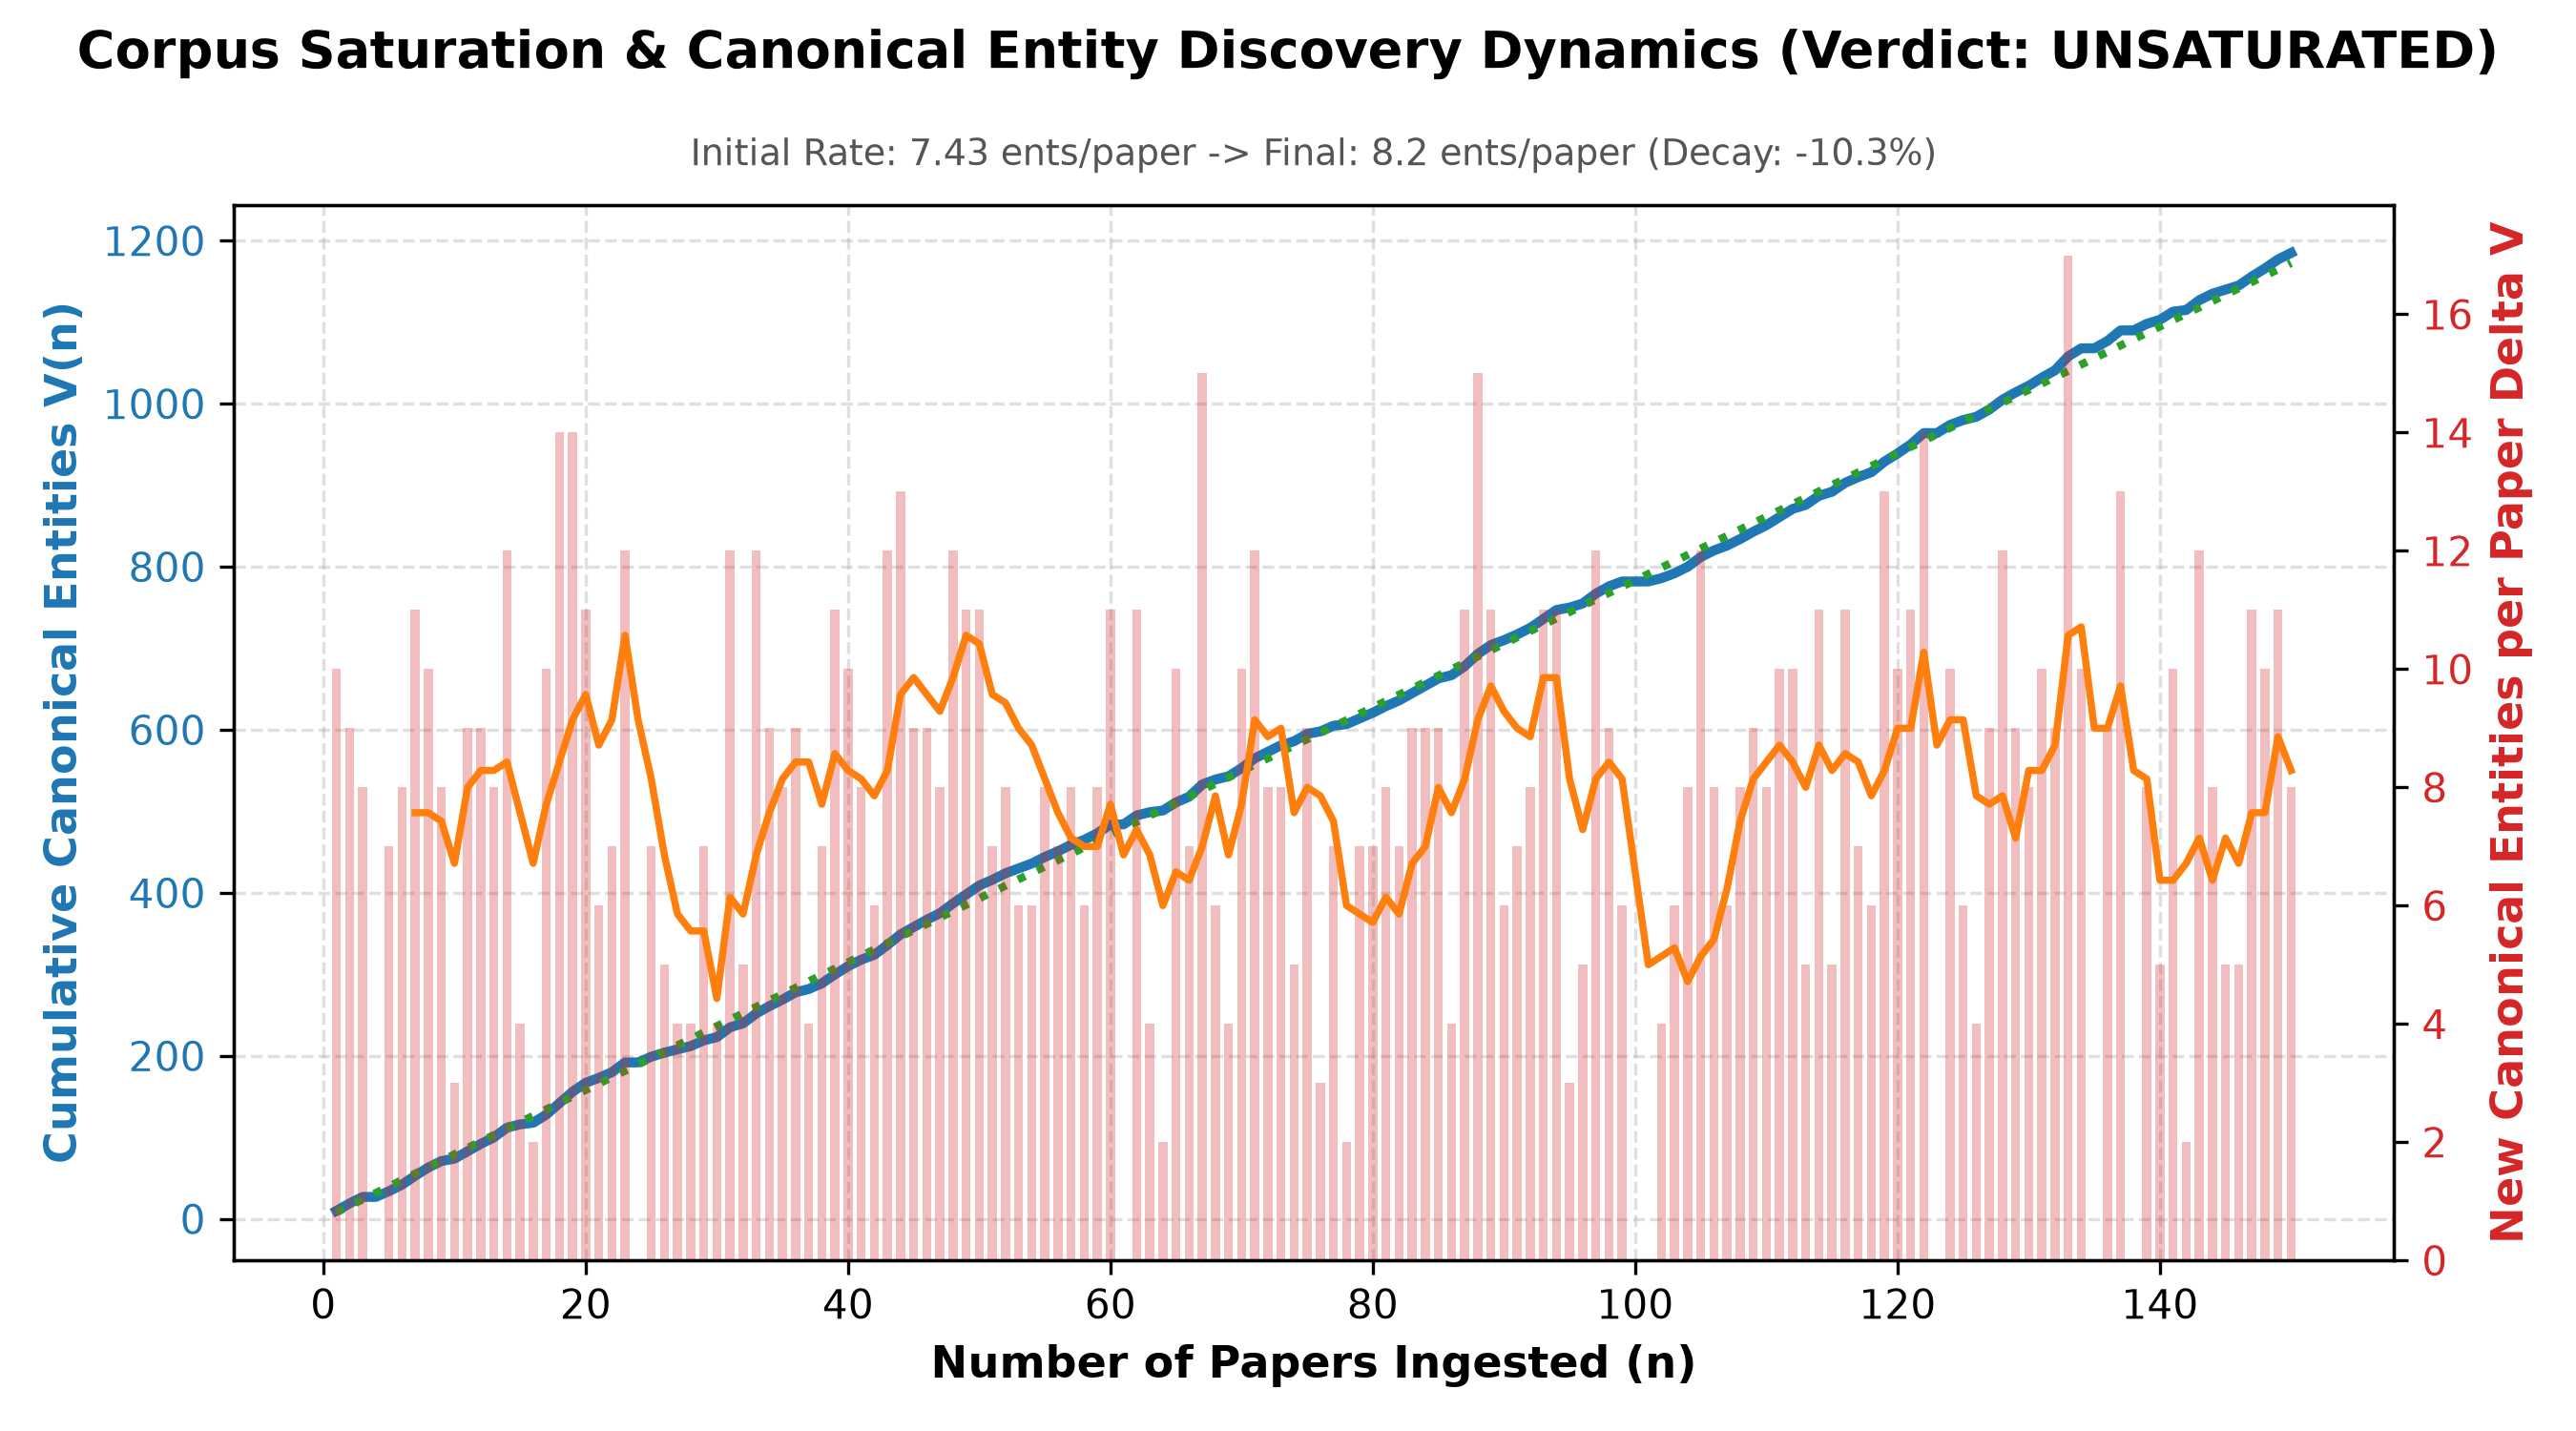
\includegraphics[width=0.44\columnwidth]{figures/corpus_saturation_curve.png}
\caption{Corpus vocabulary growth and canonical entity discovery across 150 IoT cybersecurity publications ($V_{\text{observed}}(150) = 1{,}185$). Heaps' law fit yields $\beta = 0.995$ ($R^2 = 0.9983$) and discovery decay $\Delta_{\text{decay}} = -10.3\%$, diagnosing the literature as \texttt{UNSATURATED}.}
\label{fig:saturation}
\end{figure}

Evaluating vocabulary accumulation on the canonical entity nodes of $\mathcal{G}_t$ yields $V_{\text{observed}}(150) = 1,185$ unique canonical entities. Across quintiles ($q = 30$), the initial quintile introduced $M_{\text{initial}} = 7.43$ new canonical entities per paper, while the final quintile introduced $M_{\text{final}} = 8.20$ new entities per paper. Using the marginal discovery decay metric, this yields $\Delta_{\text{decay}} = -10.3\%$. Rather than decelerating toward saturation, canonical entity discovery increased. Log-log regression yielded a Heaps' law scaling parameter of $K = 8.0315$ and growth exponent $\beta = 0.9946 \approx 0.995$ ($R^2 = 0.9983$). (Evaluating pre-canonicalization raw mentions similarly demonstrated open growth: $V = 1,396, \beta = 1.037, \Delta_{\text{decay}} = -18.6\%$). Because $\beta \ge 0.80$ and $\Delta_{\text{decay}} < 0.30$, Pillar D assigned the operational verdict \texttt{UNSATURATED}. This diagnostic prohibits claiming global scientific absence, qualifying surviving hypotheses as open-world propositions.

\subsection{Two-Stage Semantic Verification and Candidate Triage (RQ4)}
The ten local validation gates filtered initial graph signals down to five post-gate candidate hypotheses (C1--C5). Table~\ref{tab:triage} tracks these candidates across the two-stage external verification pipeline, distinguishing raw index counts from fetched and inspected records. Table~\ref{tab:evidence} presents the auditable bibliographic evidence for each candidate.

\begin{table}[htbp]
\centering
\caption{Two-Stage External Verification and Candidate Triage on Post-Gate Candidates.}
\label{tab:triage}
\scriptsize
\setlength{\tabcolsep}{2.0pt}
\begin{tabular}{p{0.5cm}p{2.6cm}ccccccp{1.7cm}p{1.3cm}}
\toprule
\textbf{ID} & \textbf{Candidate Hypothesis} & \textbf{Raw} & \textbf{Fetch} & \textbf{Insp} & \textbf{Co-M} & \textbf{Count.} & \textbf{Corrob} & \textbf{Disposition $\mathcal{D}$} & \textbf{Action $\mathcal{A}$} \\
\midrule
C1 & Deep learning IoT IDS $\rightarrow$ Zero-day attacks & 864 & 5 & 5 & 5 & 2 & 0 & \texttt{REFUTED} & \texttt{REJECT} \\
C2 & Deep learning IoT IDS $\rightarrow$ Standardized protocols & 400 & 5 & 5 & 4 & 0 & 0$^*$ & \texttt{REVIEW\_REQ} & \texttt{ABSTAIN} \\
C3 & Deep learning IoT IDS $\rightarrow$ Industrial testbeds & 146 & 5 & 5 & 4 & 2 & 0 & \texttt{REFUTED} & \texttt{REJECT} \\
C4 & ML IoT IDS $\rightarrow$ Edge computational overhead & 189 & 5 & 5 & 0 & 0 & 3 & \texttt{SUPPORTED\_}\allowbreak\texttt{OPEN} & \texttt{RETAIN\_}\allowbreak\texttt{WARN} \\
C5 & ML IoT IDS $\rightarrow$ Adversarial attack defenses & 1095 & 5 & 5 & 5 & 1 & 0 & \texttt{REFUTED} & \texttt{REJECT} \\
\bottomrule
\multicolumn{10}{p{11.5cm}}{\tiny $^*$C2 has one local corroborating citation, but it originated from the candidate's own source paper (circular provenance).}
\end{tabular}
\end{table}

\begin{table}[htbp]
\centering
\caption{Auditable Bibliographic Evidence Table for Central External and Corroborating Publications.}
\label{tab:evidence}
\tiny
\setlength{\tabcolsep}{2.5pt}
\renewcommand{\arraystretch}{0.82}
\begin{tabular}{L{0.4cm}L{1.4cm}L{2.4cm}L{2.1cm}L{4.9cm}}
\toprule
\textbf{ID} & \textbf{Citation} & \textbf{Publication Title} & \textbf{Identifier / Venue} & \textbf{Verbatim Evidence Span} \\
\midrule
C1 & Nitrat et al.~\cite{nitrat2025zeroday} & Zero-Day Attack Detection in IoT Networks\dots & DOI: 10.1109/\allowbreak OJCOMS.2025.\allowbreak 3604826 & \emph{``In zero-day scenarios, CZ-ResViT achieved 82\% accuracy on CIC IoT 2023 and 81\% on IoTID20, outperforming other DL models\dots''} \\
\midrule
C2 & Shukla et al.~\cite{shukla2025effective} & An effective hybrid deep learning metaheuristic\dots & DOI: 10.1007/\allowbreak s10791-025-\allowbreak 09708-w & \emph{``The high diversity of IoT devices, their protocols and standards, and their limited computational resources have led to the appearance of novel security challenges.''} (Supporting limitation; zero counterevidence). \\
\midrule
C3 & Ogundokun et al.~\cite{ogundokun2025litert} & LiteRT-IDSNet: A Lightweight Hybrid DL Framework\dots & DOI: 10.1109/\allowbreak ICEST66328.\allowbreak 2025.11098207 & \emph{``Experimental results show that LiteRT-IDSNet achieved training accuracy of 99.61\% and validation accuracy of 99.60\% \dots suitable real-time IIoT cybersecurity system\dots''} \\
\midrule
C4 & Jenish \& Karuppasamy~\cite{jenish2026review} & A Review on Deep Learning Techniques for Fast\dots & DOI: 10.1109/\allowbreak IDCIoT67589.\allowbreak 2026.11455671 & \emph{``\dots practical adoption is constrained by high computational overhead, inference latency, and limited interpretability.''} (Corroborating Source 1). \\
C4 & Alam et al.~\cite{alam2026reservoir} & Reservoir Computing for Network Intrusion\dots & DOI: 10.1371/\allowbreak journal.pone.\allowbreak 0355211 & \emph{``\dots high computational demands pose challenges for real-time deployment on IoT devices.''} (Corroborating Source 2). \\
C4 & Mahdi et al.~\cite{mahdi2026scf} & SCF-Net: A Lightweight Multi-Granular Feature\dots & DOI: 10.1109/\allowbreak ACCESS.2026.\allowbreak 3671487 & \emph{``\dots heavy computational cost that restricts edge application.''} (Corroborating Source 3). \\
\midrule
C5 & Nguyen et al.~\cite{nguyen2025adversarial} & Adversarial Attack and Defense in AI-Powered IDS & DOI: 10.15625/\allowbreak 1813-9663/\allowbreak 22884 & \emph{``The enhanced APELID+ achieves robust performance, maintaining 98.73\% accuracy under combined adversarial conditions\dots''} \\
\bottomrule
\end{tabular}
\end{table}

\noindent\textbf{Analysis of Candidate Triage Outcomes.} As structured in Table~\ref{tab:triage} and Table~\ref{tab:evidence}, multi-pillar verification resolved the post-gate candidates into three distinct epistemic outcomes:
(1)~\emph{Empirical Refutations (C1, C3, C5):} Despite dense lexical co-mentions, Stage~A2 confirmed recent counterevidence resolving the asserted gaps: Nitrat et al.~\cite{nitrat2025zeroday} (82\% zero-day accuracy), Ogundokun et al.~\cite{ogundokun2025litert} (99.6\% accuracy on industrial testbeds), and Nguyen et al.~\cite{nguyen2025adversarial} (98.73\% adversarial defense), yielding \texttt{REFUTED} $\rightarrow$ \texttt{REJECT}.
(2)~\emph{Circular Provenance Escalation (C2):} External literature discussed protocol diversity solely as an obstacle (e.g., Shukla et al.~\cite{shukla2025effective}) with zero counterevidence. However, Pillar~B traced the single local citation back to the candidate's own origin paper (\texttt{04b3ca64}), triggering fail-closed abstention (\texttt{REVIEW\_REQUIRED} $\rightarrow$ \texttt{ABSTAIN\_AND\_ESCALATE}).
(3)~\emph{Corroborated Open Gap (C4):} Zero counterevidence was retrieved, while Pillar~B verified three independent 2026 publications~\cite{jenish2026review,alam2026reservoir,mahdi2026scf}. Because the corpus is \texttt{UNSATURATED}, C4 was triaged as \texttt{SUPPORTED\_OPEN} $\rightarrow$ \texttt{RETAIN\_WARN}.

\noindent\textbf{Retrieval-Depth Robustness ($K_{\text{fetch}}$ Sensitivity).} In the frozen multi-provider run (Table~\ref{tab:triage}), candidate C4 was evaluated using strict canonical phrases (\emph{``machine learning-driven intrusion detection frameworks''} and \emph{``computational burdens''}) with $\tau=0.60$ token overlap, yielding 0 lexical co-mentions among the 5 fetched Semantic Scholar records (and 0 at $K=10$, 1 at $K=20$, 2 at $K=50$). To stress-test whether relaxing lexical constraints at greater retrieval depths would uncover unindexed counterevidence, a subsequent sensitivity analysis probed an expanded semantic synonym family (\emph{``machine learning''}, \emph{``intrusion detection''} and \emph{``computational overhead''}, \emph{``resource-constrained''}, \emph{``edge''}) across $K_{\text{fetch}} \in \{5, 10, 20, 50\}$ on Semantic Scholar under default relevance ranking. In this expanded-synonym run, lexical co-mentions scaled from 4 ($K=5$) to 7 ($K=10$), 13 ($K=20$), and 33 ($K=50$). At $K = 50$, neither the strict-phrase run nor the expanded-synonym run yielded verified counterevidence. In the expanded-synonym run, all 50 records were inspected; 33 passed lexical co-mention filtering, of which 18 expressed supporting limitations while the remaining 15 co-mentions were ambiguous, acknowledging edge latency bottlenecks without demonstrating resolution. Candidate C4 remained consistently \texttt{SUPPORTED\_OPEN} across $K \in \{5, 10, 20, 50\}$ under the evaluated queries and default relevance-ranking protocol.

\subsection{Pipeline Ablation Analysis (RQ5)}
Table~\ref{tab:ablation} traces the progressive filtering of candidate hypotheses across each stage of the \method{} pipeline.

\begin{table}[htbp]
\centering
\caption{Component-Level Pipeline Ablation across Post-Gate Candidates ($n = 5$).}
\label{tab:ablation}
\scriptsize
\setlength{\tabcolsep}{2.5pt}
\renewcommand{\arraystretch}{0.78}
\begin{tabular}{lccccL{3.1cm}}
\toprule
\textbf{Pipeline Stage} & \textbf{Eligible} & \textbf{Refuted} & \textbf{Review} & \textbf{Retained} & \textbf{Epistemic Triage Interpretation} \\
\midrule
1. Local Gates Only & 5 & 0 & 0 & 5 & Naive agent relying solely on graph sparsity promotes all 5 candidates. \\
2. Naive Co-Mention Baseline$^\dagger$ & 1 & 4 & 0 & 1 & Counterfactual baseline: lexical co-mention falsely refutes C2. \\
3. + Pillar A (Stage A1+A2) & 2 & 3 & 0 & 2 & Semantic verification preserves C2 as supporting limitation. \\
4. + Pillar B (Disjoint Corrob.) & 1 & 3 & 1 & 1 & Detects C2 circular citation, forcing fail-closed abstention. \\
5. + Pillars C \& D (Diagnostics) & 1 & 3 & 1 & 1$^*$ & Qualifies C4 as open-world under unsaturated corpus ($\beta=0.995$). \\
\bottomrule
\multicolumn{6}{p{\linewidth}}{\tiny $^\dagger$Counterfactual naive lexical matching rule (not \method{} policy). $^*$Retained as \texttt{SUPPORTED\_OPEN}.}
\end{tabular}
\end{table}

Without external verification, relying solely on graph sparsity prematurely promotes all five candidates. Across the cohort, external evidence refuted three candidates ($60\%$) via recent literature and prevented four ($80\%$) from unjustified promotion (three refutations and one circular-provenance abstention). Stage~A2 prevented C2 from false refutation, while Pillar~B enforced fail-closed abstention.

\subsection{Fail-Closed Fault-Injection Validation (RQ3)}
We evaluated autonomous abstention under six operational failure modes (Table~\ref{tab:fault}). Across all six predefined fault-injection scenarios ($100\%$), \method{} refrained from ungrounded claims, halting downstream execution and routing the candidate to human oversight.

\begin{table}[htbp]
\centering
\caption{Deterministic Fault-Injection Validation of the Fail-Closed Control Loop.}
\label{tab:fault}
\tiny
\setlength{\tabcolsep}{1.6pt}
\renewcommand{\arraystretch}{0.70}
\begin{tabular}{L{1.6cm}L{3.3cm}L{2.2cm}L{2.7cm}c}
\toprule
\textbf{Failure Scenario} & \textbf{Injected Condition} & \textbf{Disposition $\mathcal{D}$} & \textbf{Action $\mathcal{A}$} & \textbf{Passed} \\
\midrule
1. Index Timeout & S2/OpenAlex timeout after retries & \texttt{REVIEW\_REQUIRED} & \texttt{ABSTAIN\_AND\_ESCALATE} & \checkmark \\
2. HTTP 429 Throttle & Scholarly rate limits exhausted & \texttt{REVIEW\_REQUIRED} & \texttt{ABSTAIN\_AND\_ESCALATE} & \checkmark \\
3. Incomplete Pagination & API stream terminates prematurely & \texttt{REVIEW\_REQUIRED} & \texttt{ABSTAIN\_AND\_ESCALATE} & \checkmark \\
4. Malformed Response & Corrupted JSON or missing keys & \texttt{REVIEW\_REQUIRED} & \texttt{ABSTAIN\_AND\_ESCALATE} & \checkmark \\
5. Circular Corroboration & Only self-citations in provenance & \texttt{REVIEW\_REQUIRED} & \texttt{ABSTAIN\_AND\_ESCALATE} & \checkmark \\
6. Missing Evidence Text & Extraction lacks verbatim span & \texttt{REVIEW\_REQUIRED} & \texttt{ABSTAIN\_AND\_ESCALATE} & \checkmark \\
\midrule
\multicolumn{5}{p{\linewidth}}{\textbf{Observed Result:} 6/6 predefined fault-injection scenarios ($100\%$) produced \texttt{REVIEW\_REQUIRED} and \texttt{ABSTAIN\_AND\_ESCALATE}.} \\
\bottomrule
\end{tabular}
\end{table}

\subsection{Evidence-Supported Agenda Formulation (Candidate C4)}
For surviving candidate C4 (computational overhead and inference latency of ML models on resource-constrained IoT edge devices), \method{} formulated an actionable research agenda. To avoid generative hallucination, performance metrics are designated as \textbf{illustrative expert-review targets}, grounding the agenda in qualitative challenges cited by Jenish \& Karuppasamy~\cite{jenish2026review}, Alam et al.~\cite{alam2026reservoir}, and Mahdi et al.~\cite{mahdi2026scf}: lightweight neural architectures that preserve detection accuracy while minimizing memory footprint and inference latency on edge microcontrollers.

\section{Discussion and Sensitivity Analysis}
\label{sec:discussion}

\noindent\textbf{Heaps' Law Parameter Sensitivity.} Corpus coverage classification was evaluated across $\beta_{\text{thresh}} \in [0.65, 0.85]$ and $\Delta_{\text{decay, thresh}} \in [0.10, 0.40]$. Across all configurations, empirical values ($\beta = 0.995, \Delta_{\text{decay}} = -10.3\%$) remained strictly in the \texttt{UNSATURATED} region, confirming classification invariance.

\noindent\textbf{Summary of Empirical Findings.} (1)~RQ1 and RQ2 confirm that link absence cannot be equated with scientific absence, given an extraction miss rate of $22.2\%$ on $\mathcal{D}_{\text{gold}}$ and an unsaturated corpus ($\beta = 0.995, \Delta_{\text{decay}} = -10.3\%$). (2)~RQ4 and RQ5 show that multi-pillar verification prevented 80\% of candidate gaps from unjustified promotion (60\% refuted, 20\% escalated for circular provenance). (3)~RQ3 confirms 100\% fail-closed abstention across all six operational failure modes (Table~\ref{tab:fault}), ensuring that faults trigger human escalation rather than generative hallucination.

\section{Threats to Validity and Limitations}
\label{sec:threats}

\noindent\textbf{Diagnostics, Verification, and Canonicalization.} Gold benchmark $\mathcal{D}_{\text{gold}}$ (36 triples, 10 abstracts) demonstrates that extraction error is non-zero, rather than providing a universal bound across disciplines. Furthermore, Stage~A2 semantic verification has not yet been evaluated against an independent, human-annotated external-evidence benchmark; classification error could alter candidate labeling between \texttt{REFUTED} and supporting or ambiguous categories, and model-reported confidence values are not calibrated probabilities. In addition, boolean query generation and entity canonicalization rely on lexical normalization and TF-IDF similarity, which are vulnerable to synonym drift, abbreviations, and terminology fragmentation across subfields.

\noindent\textbf{Retrieval Scope, Scale, and Temporal Bounds.} Scholarly APIs (Semantic Scholar, OpenAlex) and top-$K$ rankings are not exhaustive, though our $K_{\text{fetch}}$ sensitivity analysis confirmed C4 stability up to $K=50$ under default ranking. Our empirical evaluation examined $n=5$ post-gate hypotheses across 150 IoT cybersecurity papers; reported triage proportions ($60\%$ refuted, $80\%$ prevented from promotion) are descriptive case-study statistics rather than population estimates, and cross-domain generalization remains unevaluated. External probes analyzed titles and abstracts, potentially omitting evidence reported solely in full text or appendices. Finally, gap triage reflects timestamped literature states that evolve as new publications appear.

\section{Conclusion}
\label{sec:conclusion}

We presented \textbf{\method{}}, an auditable autonomous reasoning architecture for evidence-grounded hypothesis triage. By executing an active epistemic control loop with Four-Pillar Evidence Verification, \method{} replaces graph sparsity heuristics with empirical verification. In an empirical case study on deep-learning IoT intrusion detection (150 publications, 1,404 relation events), \method{} refuted three candidate gaps via verified counterevidence ($60\%$), escalated circular provenance to human review, and qualified an edge-computing gap corroborated by independent literature. Across six predefined fault-injection scenarios, the architecture enforced fail-closed abstention without ungrounded conjecture, demonstrating how explicit epistemic constraints prevent autonomous scientific reasoning pipelines from promoting unsupported hypotheses when evidence is incomplete, contradictory, or provenance-limited.

\bibliographystyle{splncs04}
\bibliography{references}

\end{document}
